\documentclass[titlepage]{article}
\usepackage{babel}
\usepackage{amsmath}
\usepackage{amssymb}
\usepackage{amsthm}
\usepackage{multicol} %spalten in seite
\usepackage{graphicx} %bilder einfügen
\usepackage[normalem]{ulem} %durchstreichen
\usepackage{tabto} %tabulator mit \tab
\usepackage{hyperref}
\usepackage{tikz}
\usetikzlibrary{shapes.geometric}
\usepackage{wasysym}
\usepackage{bbm}
\usepackage{bbold}
\usepackage{xcolor}
\usepackage[T1]{fontenc}
\usepackage{mathrsfs}  
\usepackage[utf8]{inputenc}
\usepackage{listings} %quellcode
\pagestyle{plain}
\pagenumbering{arabic}
\renewcommand{\arraystretch}{1.3} %vertikaler abstand von tabellen
\newcommand{\n}{\newline}
\usepackage[left=20mm, right=15mm, top=15mm, bottom=15mm, paper=a4paper]{geometry}
\renewcommand{\contentsname}{Inhaltsverzeichnis}

\newcommand{\K}{\mathbb{K}}
\newcommand{\C}{\mathbb{C}}
\newcommand{\N}{\mathbb{N}}
\newcommand{\Q}{\mathbb{Q}}
\newcommand{\R}{\mathbb{R}}
\newcommand{\1}{\mathbb{1}}
\newcommand{\0}{\mathbb{0}}
\newcommand{\Z}{\mathbb{Z}}

\newcommand{\vecD}[3]{\left(\begin{smallmatrix}#1\\#2\\#3\end{smallmatrix}\right)}
\newcommand{\matrixZ}[4]{\begin{pmatrix}#1&#2\\#3&#4\end{pmatrix}}
\newcommand{\detZ}[4]{\begin{vmatrix}#1&#2\\#3&#4\end{vmatrix}}
\newcommand{\smallMatrixZ}[4]{\left(\begin{smallmatrix}#1&#2\\#3&#4\end{smallmatrix}\right)}
\newcommand{\smallDetZ}[4]{\left|\begin{smallmatrix}#1&#2\\#3&#4\end{smallmatrix}\right|}
\newcommand{\vecZ}[2]{\left(\begin{smallmatrix}#1\\#2\end{smallmatrix}\right)}
\newcommand{\detD}[9]{\begin{vmatrix}#1&#2&#3\\#4&#5&#6\\#7&#8&#9\end{vmatrix}}
\newcommand{\matrixD}[9]{\begin{pmatrix}#1&#2&#3\\#4&#5&#6\\#7&#8&#9\end{pmatrix}}

\newcommand{\sarrusD}[9]{(#1)\cdot(#5)\cdot(#9)+(#4)\cdot(#8)\cdot(#3)+(#7)\cdot(#2)\cdot(#6)-(#7)\cdot(#5)\cdot(#3)-(#1)\cdot(#8)\cdot(#6)-(#4)\cdot(#2)\cdot(#9)}

\newcommand{\kreuzproduktD}[6]{\left(\begin{matrix}#2#6-#3#5\\#3#4-#1#6\\#1#5-#2#4\end{matrix}\right)}

\begin{document}
	
	\begin{center}
		
\begin{tikzpicture}
			\draw (0,0) node[draw, rectangle]{\textsc{Wintersemester 2020/21}};
		\end{tikzpicture}
		\hrulefill\\
		\begin{center}
			\LARGE\textsc{Lineare Algebra - Übung 11} \normalsize\\
		\end{center}
		\hrulefill
		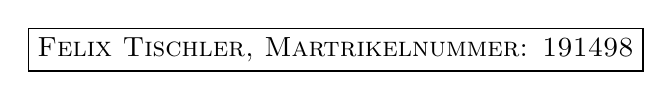
\begin{tikzpicture}
			\draw (0,0) node[draw, rectangle]{\textsc{Felix Tischler, Martrikelnummer: 191498}};
		\end{tikzpicture}
		\date{\today}
	\end{center}

	\paragraph{Hausaufgabe 11.1:}3$\times$3 Determinanten
		\begin{align*}
			\textit{Sei }&A:=\matrixD{x_1}{y_1}{z_1}{x_2}{y_2}{z_2}{x_3}{y_3}{z_3}\textit{ dann }&\detD{x_1}{y_1}{z_1}{x_2}{y_2}{z_2}{x_3}{y_3}{z_3}\overset{laplace}{\Rightarrow}x_1\cdot\detZ{y_2}{z_2}{y_3}{z_3}-x_2\cdot\detZ{y_1}{z_1}{y_3}{z_3}+x_3\cdot\detZ{y_1}{z_1}{y_2}{z_2}\\
			&&=x_1(y_2z_3-y_3z_2)-x_2(y_1z_3-y_3z_1)+x_3(y_1z_2-y_2z_1)\\
			&&=\underbrace{x_1(y_2z_3-y_3z_2)+x_2(y_3z_1-y_1z_3)+x_3(y_1z_2-y_2z_1)}_\varXi
		\end{align*}
		\begin{align*}
			<\vec{x}\mid(\vec{y}\times\vec{z})>&=\sum_{i=1}^{m}\vec{x}(\vec{y}\times\vec{z})=(\vec{y}\times\vec{z})^T\cdot\vec{x}=(y_2z_3-y_3z_2\quad y_3z_1-y_1z_3\quad y_1z_2-y_2z_1)\cdot\vecD{x_1}{x_2}{x_3}\\
			&=x_1(y_2z_3-y_3z_2)+x_2(y_3z_1-y_1z_3)+x_3(y_1z_2-y_2z_1)=\varXi\qed
		\end{align*}\\
		D.h. $\underbrace{\langle\vec{x}\mid(\vec{y}\times\vec{z})\rangle=det(\vec{x},\vec{y},\vec{z})}_\kappa$\\\\
		Wenn $[\vec{y},\vec{z}]$ lin. unabhängig, dann $\vec{y}\times\vec{z}\neq\vec{0}$:
		\begin{align*}
			&\textit{Wenn }\vec{y},\vec{z}\textit{ lin. unabhängig, dann: }\underbrace{\vec{z}\neq\lambda\cdot\vec{y}}_\varkappa\textit{ mit }\lambda\in\K.\\
			&(\vec{y}\times\vec{z})=\kreuzproduktD{y_1}{y_2}{y_3}{z_1}{z_2}{z_3}\overset{\varkappa}{\neq}\kreuzproduktD{y_1}{y_2}{y_3}{\lambda\cdot y_1}{\lambda\cdot y_2}{\lambda\cdot y_3}=\vec{0}
		\end{align*}
		Wenn $\vec{y}\times\vec{z}\neq\vec{0}$, dann $[\vec{y},\vec{z}]$ lin. unabhängig:
		\begin{align*}
			&\textit{Sei }\vec{y}\times\vec{z}=\vec{x}\mid\textit{ $\vec{x}$ ist lin. unabhängig zu }\vec{y},\vec{z}.\\
			&\langle\vec{x}\mid(\vec{y}\times\vec{z})\rangle=\langle\vec{x}\mid\vec{x}\rangle\overset{\kappa}{\Rightarrow}||\vec{y}\times\vec{z}||^2\\
			&\vec{y}\times\vec{z}\neq\vec{0}
			\Rightarrow||\vec{y}\times\vec{z}||\neq0
			\Rightarrow||\vec{y}\times\vec{z}||^2>0\\
			&\overset{\kappa}{\Rightarrow} det(\vec{x},\vec{y},\vec{z})>0\Rightarrow\vec{y},\vec{z}\textit{ sind lin. unabhängig zueinander.}\qed
		\end{align*}
		D.h. $[\vec{y},\vec{z}]$ ist genau dann lin. unabhängig, wenn $\vec{y}\times\vec{z}\neq0$

	\paragraph{Hausaufgabe 11.2: } Längen/Winkel
		\begin{align*}
			&||\vec{a}||=\sqrt{<\vec{a}\mid\vec{a}>}=\sqrt{\vec{a}^T\cdot\vec{a}}=\sqrt{\vecD{3}{-4}{12}\cdot(3\quad-4\quad12)}=\sqrt{169}=13\\
			&||\vec{b}||=\sqrt{<\vec{b}\mid\vec{b}>}=\sqrt{\vec{b}^T\cdot\vec{b}}=\sqrt{\vecD{12\sqrt{3}}{-3\sqrt{3}}{-4\sqrt{3}}\cdot(12\sqrt{3}\quad-3\sqrt{3}\quad-4\sqrt{3})}=\sqrt{507}=13\sqrt{3}\\
			&||\vec{c}||=\sqrt{<\vec{c}\mid\vec{c}>}=\sqrt{\vec{c}^T\cdot\vec{c}}=\sqrt{\vecD{-3-12\sqrt{3}}{4+3\sqrt{3}}{-12+4\sqrt{3}}\cdot(-3-12\sqrt{3}\quad4+3\sqrt{3}\quad-12+4\sqrt{3})}=\sqrt{676}=26\\\\
			&<\vec{a}\mid\vec{b}>=\vec{b}^T\cdot\vec{a}=0\\
			&<\vec{a}\mid\vec{c}>=\vec{c}^T\cdot\vec{a}=-169\\
			&<\vec{b}\mid\vec{c}>=\vec{c}^T\cdot\vec{b}=-507\\\\
			&\sphericalangle(\vec{a},\vec{b})=\arccos\frac{<\vec{a}\mid\vec{b}>}{||\vec{a}||\cdot||\vec{b}||}=\arccos\frac{0}{13\cdot13\sqrt{3}}=\frac{1}{2}\pi\\
			&\sphericalangle(\vec{a},\vec{c})=\arccos\frac{<\vec{a}\mid\vec{c}>}{||\vec{a}||\cdot||\vec{c}||}=\arccos\frac{-169}{13\cdot26}=\frac{2}{3}\pi\\
			&\sphericalangle(\vec{b},\vec{c})=\arccos\frac{<\vec{b}\mid\vec{c}>}{||\vec{b}||\cdot||\vec{c}||}=\arccos\frac{-507}{13\sqrt{3}\cdot26}=\frac{5}{6}\pi
		\end{align*}
	
	\newpage
	\paragraph{Hausaufgabe 11.3:} Prüfen Sie, ob die angegebene Matrix über $\R$ diagonalisierbar ist und bestimmen Sie ggf. eine diagonalisierende Matrix.\\\\
		(a)
			\begin{align*}
				&A:=\matrixZ{1}{3}{3}{1}\textit{, A ist symmetrisch }\Rightarrow\textit{ A ist diagonalisierbar.}\\
				&\textit{Eigenwerte: }\\
				&\quad\quad\lambda\textit{ ist Eigenwert von A }\Leftrightarrow det(X\1-A)=0\\
				&\quad\quad\detZ{X-1}{-3}{-3}{X-1}=0\overset{sarrus}{\Rightarrow}(X-1)^2-9=0\\
				&\quad\quad\overset{pq}{\Rightarrow}\lambda_1=1+\sqrt{9}=-2\textit{ und }\lambda_2=1-\sqrt{9}=4\\
				&\textit{Eigenvektoren: }\\
				&\quad\quad\lambda_1:\\
				&\quad\quad\quad
				\left(\begin{array}{cc|c}
					-3&-3&0\\-3&-3&0
				\end{array}\right)
				\rightsquigarrow
				\left(\begin{array}{cc|c}
					1&1&0\\0&0&0
				\end{array}\right)
				\Rightarrow E_{\lambda_1}=Span(\vecZ{-1}{1})\\
				&\quad\quad\lambda_2:\\
				&\quad\quad\quad
				\left(\begin{array}{cc|c}
					3&-3&0\\-3&3&0
				\end{array}\right)
				\rightsquigarrow
				\left(\begin{array}{cc|c}
					1&-1&0\\0&0&0
				\end{array}\right)
				\Rightarrow E_{\lambda_2}=Span(\vecZ{1}{1})\\\\
				&\quad\quad\Rightarrow S=(\vecZ{-1}{1},\vecZ{1}{1})=\textit{ diagonalisierende Matrix.}\\\\
				&\textit{Und inverse der diagonalisierenden Matrix:}\\
				&\quad\quad\quad
				\left(\begin{array}{cc|cc}
					-1&1&1&0\\1&1&0&1
				\end{array}\right)
				\overset{II+I}{\rightsquigarrow}
				\left(\begin{array}{cc|cc}
					-1&1&1&0\\0&2&1&1
				\end{array}\right)
				\overset{II:2}{\rightsquigarrow}
				\left(\begin{array}{cc|cc}
					-1&1&1&0\\0&1&1/2&1/2
				\end{array}\right)\\
				&\quad\quad\quad
				\overset{I-II}{\rightsquigarrow}
				\left(\begin{array}{cc|cc}
					-1&0&1/2&-1/2\\0&1&1/2&1/2
				\end{array}\right)
				\overset{I\cdot(-1)}{\rightsquigarrow}
				\left(\begin{array}{cc|cc}
					1&0&-1/2&1/2\\0&1&1/2&1/2
				\end{array}\right)\Rightarrow S^{-1}=\frac{1}{2}\matrixZ{-1}{1}{1}{1}
			\end{align*}
		(b)
			\begin{align*}
				&\textit{Eigenwerte: }\\
				&\quad\quad\lambda\textit{ ist Eigenwerten von }A\Leftrightarrow det(X\1-A)=0\\
				&\quad\quad\detD{X-2}{-1}{0}{-1}{X}{-2}{0}{1}{X-2}=0\xrightarrow{Spalte\,3-2\cdot Spalte\,1}\detD{X-2}{-1}{-2(X-2)}{-1}{X}{0}{0}{1}{X-2}=0\\
				&\quad\quad\xrightarrow{I+2\cdot III}\detD{X-2}{1}{0}{-1}{X}{0}{0}{1}{X-2}=0\overset{Laplace}{\Rightarrow}(X-2)\cdot\detZ{X-2}{1}{-1}{X}=0\\
				&\quad\quad\overset{Sarrus}{\Rightarrow}(X-2)(X^2-2X+1)=0=(X-2)(X-1)^2\Rightarrow\lambda_1=2,\lambda_{2,3}=1\\
				&\textit{Eigenvektoren: }\\
				&\quad\quad\lambda_1:\\
				&\quad\quad
				\left(\begin{array}{ccc|c}
					0&-1&0&0\\-1&2&-2&0\\0&1&0&0
				\end{array}\right)\Rightarrow E_{\lambda_1}=Span(\vecD{-2}{0}{1})\\
				&\quad\quad\lambda_{2,3}:\\
				&\quad\quad
				\left(\begin{array}{ccc|c}
					-1&-1&0&0\\-1&1&-2&0\\0&1&-1&0
				\end{array}\right)\xrightarrow{I\cdot(-1)}
				\left(\begin{array}{ccc|c}
					1&1&0&0\\-1&1&-2&0\\0&1&-1&0
				\end{array}\right)\xrightarrow{II+I}
				\left(\begin{array}{ccc|c}
					1&1&0&0\\0&2&-2&0\\0&1&-1&0
				\end{array}\right)\\
				&\quad\quad E_{\lambda_{2,3}}=Span(\vecD{-1}{1}{1})\\
				&\quad\quad\sum_{i=1}^{3}dim\,E_{\lambda_i}(A)=2\Rightarrow\textit{geometrische Vielfachheit $<$ algebr. Vielfachheit}\\
				&\quad\quad\Rightarrow\textit{nicht diagonalisierbar!}
			\end{align*}
		(c)
			\begin{align*}
				&\textit{Eigenwerte: }\\
				&\quad\quad\lambda\textit{ ist Eigenwerten von }A\Leftrightarrow det(X\1-A)=0\\
				&\quad\quad\detD{X-3}{10}{10}{0}{X-3}{0}{0}{5}{X+2}=0\overset{laplace}{\Rightarrow}(X-3)\cdot\detZ{X-3}{0}{5}{X+2}=0\\
				&\quad\quad\overset{sarrus}{\Rightarrow}(X-3)(X-3)(X+2)=0\Rightarrow\lambda_{1,2}=3,\lambda_3=-2\\
				&\textit{Eigenvektoren: }\\
				&\quad\quad\lambda_{1,2}:\\
				&\quad\quad
				\left(\begin{array}{ccc|c}
					0&10&10&0\\0&0&0&0\\0&5&5&0
				\end{array}\right)
				\Rightarrow E_{\lambda_{1,2}}=Span(\vecD{0}{-1}{1},\vecD{1}{0}{0})\\
				&\quad\quad\lambda_3:\\
				&\quad\quad\left(\begin{array}{ccc|c}
					-5&10&10&0\\0&-5&0&0\\0&5&0&0
				\end{array}\right)
				\Rightarrow E_{\lambda_3}=Span(\vecD{2}{0}{1})\\\\
				&\quad\quad\Rightarrow S=(\vecD{0}{1}{-1},\vecD{1}{0}{0},\vecD{2}{0}{1})\\
				&\textit{Und inverse der diagonalisierenden Matrix:}\\
				&\quad\quad\matrixD{0}{1}{2}{1}{0}{0}{-1}{0}{1}\matrixD{a}{b}{c}{d}{e}{f}{g}{h}{i}=\matrixD{1}{0}{0}{0}{1}{0}{0}{0}{1}\\
				&\quad\quad\matrixD{d+2g}{e+2h}{f+2i}{a}{b}{c}{-a+g}{-b+h}{-c+1}=\matrixD{1}{0}{0}{0}{1}{0}{0}{0}{1}\\
				&\quad\quad\Rightarrow a=c=g=0\\
				&\quad\quad\Rightarrow b=i=d=h=1\\
				&\quad\quad\Rightarrow f=e=-2\\
				&\quad\quad\Rightarrow S^{-1}=\matrixD{0}{1}{0}{1}{-2}{-2}{0}{1}{1}\\
			\end{align*}\
	
\end{document}
